\documentclass[11pt]{article}
\usepackage[a4paper,margin=0.7in]{geometry}
\usepackage[T1]{fontenc}
\usepackage[utf8]{inputenc}
\usepackage{lmodern}
\usepackage{graphicx}
\usepackage{pdflscape}
\usepackage{longtable}
\usepackage{booktabs}
\usepackage{array}
\usepackage{hyperref}
\usepackage{xcolor}
\newcolumntype{L}[1]{>{\raggedright\arraybackslash}p{#1}}
\hypersetup{colorlinks=true,linkcolor=blue,urlcolor=blue}
\title{High-level Implementation Graph for \texttt{experiments\_related}}
\author{Generated from the implementation-only export}
\date{July 7, 2026}
\begin{document}
\maketitle

\paragraph{Scope.} This graph is reconstructed from the uploaded implementation-only archive rooted at \path{experiments_related}. It maps implementation families and staged artifacts only; it does not claim that any training run completed or that any reported numerical metric was achieved.

\paragraph{Edge semantics.} Solid edges denote direct script/module wiring, explicit imports, launch calls, or direct data loading conventions visible in code. Dashed edges denote staged filesystem dependencies inferred from output/checkpoint paths, CLI arguments, or wrapper scripts; the archive does not include the produced artifacts.

\begin{landscape}
\begin{figure}[p]
\centering
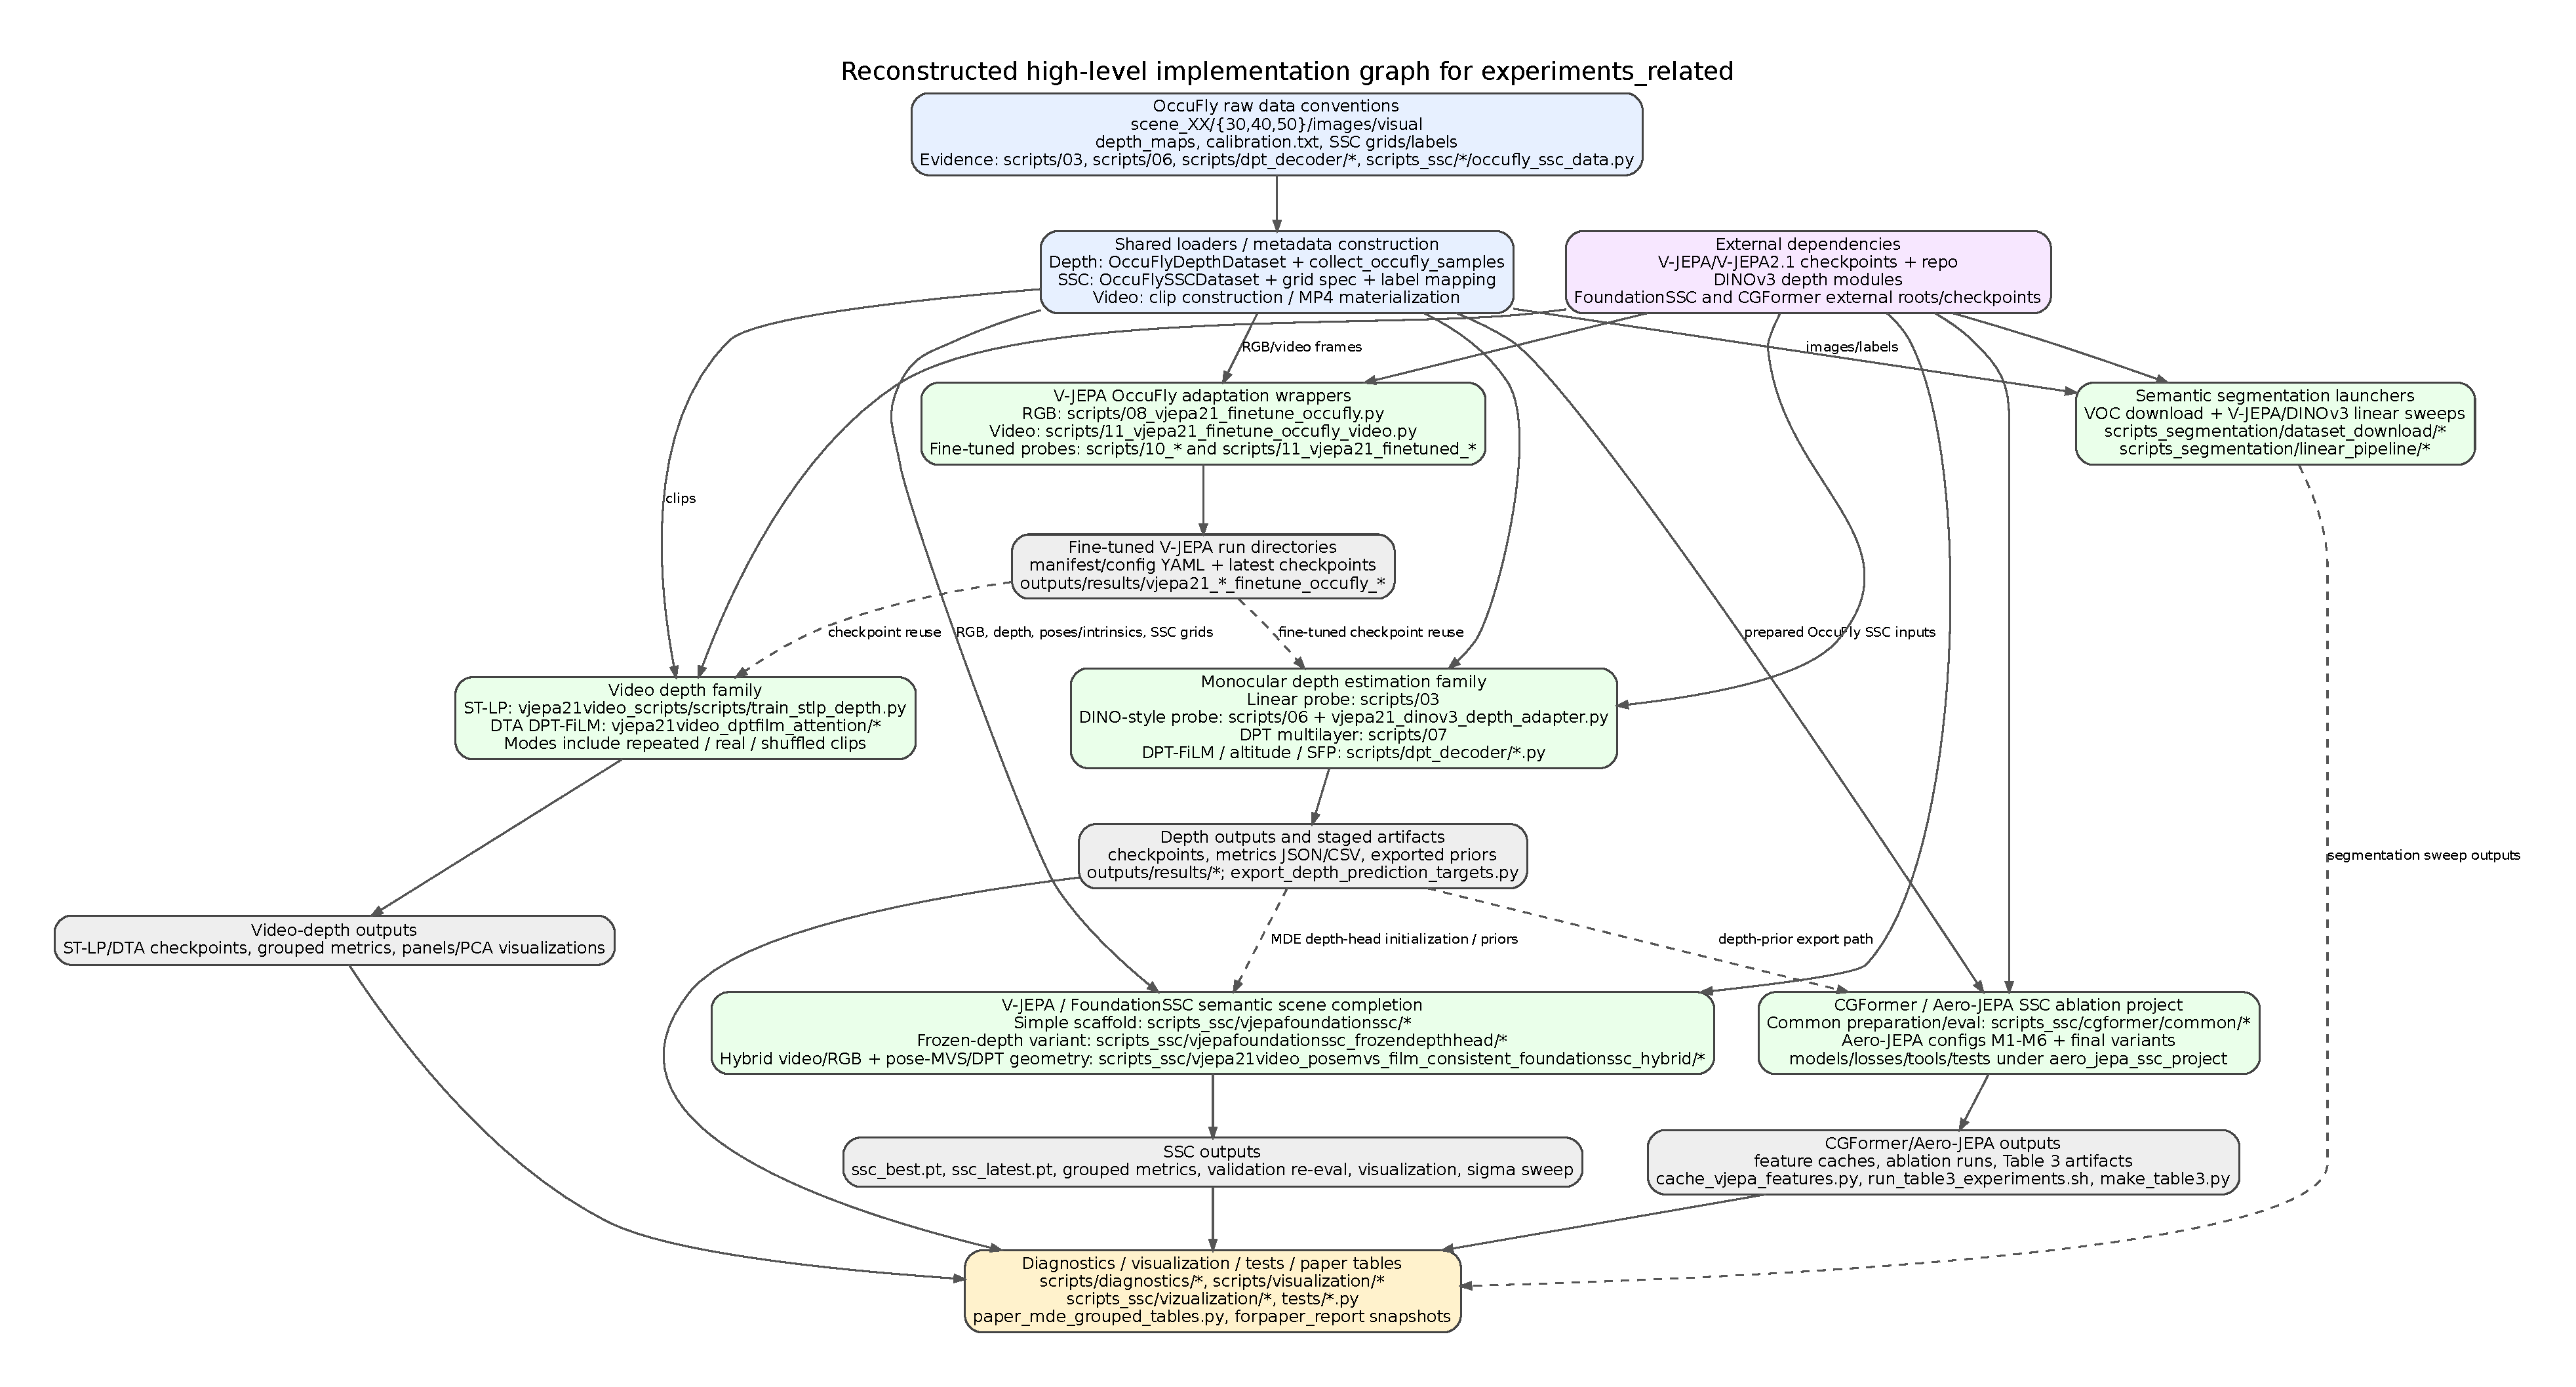
\includegraphics[width=\linewidth,height=0.92\textheight,keepaspectratio]{implementation_graph_overview_compact.pdf}
\caption{Reconstructed high-level implementation graph. Node labels include the primary source paths used as evidence.}
\end{figure}
\end{landscape}

\section*{Evidence table}
\begin{longtable}{L{0.28\linewidth}L{0.66\linewidth}}
\toprule
Graph element & Primary source paths \\
\midrule
\endhead
OccuFly data conventions & \path{scripts/03_train_vjepa_linear_depth.py}; \path{scripts/06_vjepa21_dinov3_linearprobe_occufly.py}; \path{scripts/dpt_decoder/train_vjepa21_vitG_dpt_film_occufly.py}; \path{scripts_ssc/*/vjepafoundationssc/occufly_ssc_data.py}; \path{scripts_ssc/*/occufly_grid_config.json}. \\
Shared loaders and metadata & \path{scripts/03_train_vjepa_linear_depth.py}; \path{scripts/06_vjepa21_dinov3_linearprobe_occufly.py}; \path{scripts/07_vjepa21_dinov3_DPT_multilayer_decoder_occufly.py}; \path{scripts/dpt_decoder/*.py}; \path{vjepa21video_scripts/src/vjepa21video_depth/*}; \path{scripts_ssc/*/vjepafoundationssc/occufly_ssc_data.py}. \\
External dependencies & \path{scripts/08_vjepa21_finetune_occufly.py}; \path{scripts/11_vjepa21_finetune_occufly_video.py}; \path{scripts/06_vjepa21_dinov3_linearprobe_occufly.py}; \path{scripts/07_vjepa21_dinov3_DPT_multilayer_decoder_occufly.py}; \path{scripts_ssc/*/vjepafoundationssc/repo_paths.py}; \path{scripts_ssc/*/vjepafoundationssc/foundation_ssc/real_adapters.py}; \path{scripts_ssc/cgformer/common/*}. \\
MDE family & \path{scripts/03_train_vjepa_linear_depth.py}; \path{scripts/06_vjepa21_dinov3_linearprobe_occufly.py}; \path{scripts/vjepa21_dinov3_depth_adapter.py}; \path{scripts/07_vjepa21_dinov3_DPT_multilayer_decoder_occufly.py}; \path{scripts/dpt_decoder/train_vjepa21_vitG_dpt_film_occufly.py}; \path{scripts/dpt_decoder/train_vjepa21_vitG_dpt_altitude_feature_occufly.py}; \path{scripts/dpt_decoder/train_vjepa21_vitG_final_sfp_dpt_film_occufly.py}. \\
V-JEPA adaptation & \path{scripts/08_vjepa21_finetune_occufly.py}; \path{scripts/11_vjepa21_finetune_occufly_video.py}; \path{scripts/10_vjepa21_finetuned_linearprobe_occufly.py}; \path{scripts/11_vjepa21_finetuned_DPT_multilayer_decoder_occufly.py}; \path{scripts/run_finetuned_video_*_sweep_ddp.sh}. \\
Video depth & \path{vjepa21video_scripts/scripts/train_stlp_depth.py}; \path{vjepa21video_scripts/src/vjepa21video_depth/*}; \path{vjepa21video_scripts/vjepa21video_dptfilm_attention/scripts/train_video_dptfilm_attention.py}; \path{vjepa21video_scripts/vjepa21video_dptfilm_attention/src/vjepa21video_dptfilm_attention/*}. \\
Semantic segmentation & \path{scripts_segmentation/dataset_download/download_voc12.sh}; \path{scripts_segmentation/linear_pipeline/run_vjepa21_voc12_linear_sweep.sh}; \path{scripts_segmentation/linear_pipeline/run_vjepa21_occufly_linear_sweep.sh}; \path{scripts_segmentation/linear_pipeline/occufly_21class_label_map.json}. \\
V-JEPA/FoundationSSC SSC & \path{scripts_ssc/vjepafoundationssc/*}; \path{scripts_ssc/vjepafoundationssc_frozendepthhead/*}; \path{scripts_ssc/vjepa21video_posemvs_film_consistent_foundationssc_hybrid/vjepafoundationssc/train_vjepa_occufly_ssc.py}; \path{scripts_ssc/vjepa21video_posemvs_film_consistent_foundationssc_hybrid/vjepafoundationssc/foundation_ssc/*}. \\
CGFormer/Aero-JEPA & \path{scripts_ssc/cgformer/common/*}; \path{scripts_ssc/cgformer/vitGFilmaltitudeconditioning/export_vjepa21vitGdptFilm_priors.py}; \path{scripts_ssc/cgformer/aero_jepa_ssc_project/configs/occufly/*.yaml}; \path{scripts_ssc/cgformer/aero_jepa_ssc_project/src/aero_jepa_ssc/*}; \path{scripts_ssc/cgformer/aero_jepa_ssc_project/tools/*}; \path{scripts_ssc/cgformer/aero_jepa_ssc_project/tests/*}. \\
Diagnostics, visualization, tests, reporting & \path{scripts/diagnostics/*}; \path{scripts/visualization/*}; \path{scripts/visualizations_rgv_vs_video/*}; \path{scripts_ssc/vizualization/*}; \path{tests/*.py}; \path{scripts/paper_mde_grouped_tables.py}; \path{scripts/best20rmse_mde_pipeline/update_best20rmse.py}; \path{forpaper_report/*}. \\
\bottomrule
\end{longtable}

\end{document}
